\section{Outcome diagram} \label{out_syntax}
        An abstract syntax for constructing outcome diagrams has already been defined in a previous paper \cite{art}, nevertheless, the oscilloscope needs a textual way to define an outcome diagram. \\ 
        We define  a grammar to create an outcome diagram in our oscilloscope, which is a textual interpretation of the abstract syntax.
        
      
        \subsection{Causal link}
            A causal link between two components can be defined by a right arrow from \texttt{component\_i} to \texttt{component\_j}:
        \begin{minted}{text}
            component_i -> component_j 
        \end{minted}
        
        \subsection{Sub-outcome diagrams}
            Multiple sub-outcome diagrams can be created for multiple parts of the system. They can then be linked together to form the global system outcome diagram. Sub-outcome diagrams can observe one or multiple components.
        Recall \cref{fig:probes_o}, we defined a probe which observes the sequential composition of $o_1, o_2$. The probe (sub-outcome diagram) $p_1$ can be defined as:
        \begin{minted}{text}
            p_1 = o_1 -> o_2;
        \end{minted}

        A probe is attached at the start and end events of $p_1$, it will observe the whole system and the calculated $\Delta$Q will be the convolution of $o_1, o_2$.

        The lines defining these diagrams must be semicolon terminated. Outcomes and operators cannot be defined on their own, they must be observed in a sub-outcome diagram.
        
        Sub-outcome diagrams can be reused in other diagrams by adding \texttt{s:} (sub-outcome diagram) before they are used.

            \begin{minted}{text}
                p_3 = s:p_1 -> s:p_2;
            \end{minted}
            This allows for easy composition and reuse of different parts of the system, allowing for independent refining of diagrams.

        \subsection{Outcomes}
            To attach a probe to an outcome observables, it is enough to declare an outcome with its name inside a diagram.
                \begin{minted}{text}
                    ... = outcomeName;
                \end{minted}
        \subsection{Operators}
            First-to-finish, all-to-finish and probabilistic choice operators must contain at least two components.
              \subsubsection{All-to-finish operator}
            An all-to-finish operator needs to be defined as follows:
            \begin{minted}{text}
                a:name(component1, component2...)
            \end{minted}

        \subsubsection{First-to-finish operator}
            A first-to-finish operator needs to be defined as follows:
            \begin{minted}{text}
                f:name(component1, component2...)
            \end{minted} 

        \subsubsection{Probabilistic choice operator}
            A probabilistic choice operator needs to be defined as follows:
            \begin{minted}{text}
                p:name[probability_1, probability_2, ... probability_i](component_1, component_2, ..., component_i) 
            \end{minted}
            In addition to being comma separated, the number of probabilities inside the brackets must match the number of components inside the parentheses. For $n$ probabilites $p_i$, $0 < p_i < 1$, $\sum_{i = 0}^{n} p_i = 1$ 
        
            
        \subsection{Limitations}
            Our system has a few limitations compared to the theoretical applications of $\Delta$Q, namely, no cycles are allowed in the definition of outcome diagrams. 
        
        \begin{minted}{text}
            p_1 = s:p_2;
            p_2 = s:p_1;
        \end{minted}
        The above example is not allowed and will raise an error when defined.  

    \subsection{Outcome diagram example}
        We provide a sample example of an outcome diagram definition. We also provide its resulting outcome diagram with probes inserted.
        \begin{figure}[H]
        \begin{minted}{text}
            two_hops = o2 -> o3;
            total = p:pc[0.9, 0.1](o1, s:two_hops);
        \end{minted}
            \caption{Sample textual definition of an outcome diagram.}
        \label{fig:outcd}
        \end{figure}

        \begin{figure}[H]
            \begin{center}
                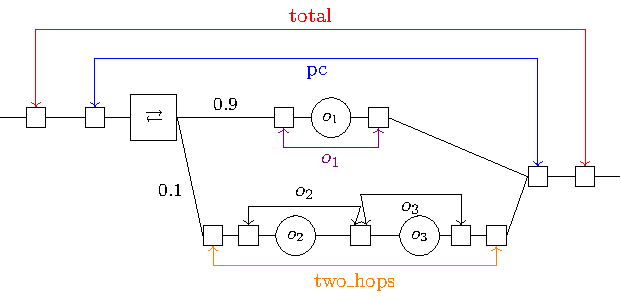
\includegraphics[scale=1.3]{tikz/system.pdf}
            \end{center}
            \caption{Resulting outcome diagram for definition \ref{fig:outcd}.}%
        \end{figure}
